\title{A title}
\date{\vspace{-5ex}}
\documentclass[12pt]{article}
\usepackage{amsmath}
\usepackage{mathabx}
\usepackage{graphics}
\usepackage[top=0.75in, bottom=0.75in, left=1in, right=1in]{geometry}
\usepackage{tabu}
\usepackage[english]{babel}
\usepackage{natbib}
\bibliographystyle{evolution}
\usepackage{rotating}
\usepackage[capitalize, sort&compress]{cleveref}
\usepackage{float}
%\newcommand{\crefrangeconjunction}{--}
%\crefname{section}{Sect.}{Sects.}
%\crefname{equation}{Eq.}{Eqs.}
%\crefformat{equation}{Eq.~#2#1#3}
%\crefrangeformat{equation}{Eqs.~#3#1#4--#5#2#6}
%\crefmultiformat{equation}{Eqs.~#2#1#3}{--#2#1#3}{, #2#1#3}{ and~#2#1#3}
 
% for comments visible in the compiled pdf
%\usepackage{color}
%\definecolor{orange}{rgb}{0.8,0.4,0}
%\newcommand{\eeg}[1]{{\em \color{orange} #1}}

% Tell latex how it can introduce linebreaks if necessary.
\hyphenation{Bar-thol-o-mew}

\begin{document}
\maketitle 

\section*{Introduction}
Niche is one of the most important concepts in ecology.
Niche links how an individual interacts with its external environment and thus determines its temporal and spatial distribution and abundance.
The niche concept became popular with the work of Hutchinson who defined species' niche as a hypervolume in an n-dimensional space (ref).
Although the exact meaning of what a dimension is unclear (e.g., Abrams, Chase and Leibold), the geometrical abstraction helps to visualize two important properties of the niche.
First, the location (center) of the hypervolume in the space that defines where performance is maximal.
Second, the width of the hypervolume that defines the range of conditions an individual can persist in. 
Defining these two properties for a given species has become a central focus for both empirical and theoretical works.


Empirical studies derived the niche of the species by correlating current occurrence with the environmental conditions it occurs. 
This approach is one of the most important tools for predicting the effect of climate change on species' future distribution and persistence simply by intersecting the future environmental conditions with the previously measured niche (refs.).
A more direct empirical approach is to measure experimentally the performance of individuals (refs).
In that approach, one focuses usually one dimension---a slice of the hypervolume.
One of the best example is to measure performance along temperature gradient. 
In general, species responds in a non-monotonic way to temperature and is often skewed to the left (refs).

At the other end of the spectrum, mathematical models make assumptions about niche rather than deriving it. 
MacArthur and Levins assumed that resource utilization curve follows a normal distribution, such choice is often for mathematical convenience although the best statistical fit for some performances is a normal distribution (Angiletta2006). 
A good mix between theoretical and empirical approach is to use energy to construct the niche (refs).
These energy budget models aim to quantify the net energy gain of an individual by modeling the energetic gain through foraging minus the cost for maintenance and survival.
It is mechanistic and realistic in the sense that energy is modeled even at the molecular level and use first principles in thermodynamics, morphology, physiology and ecology.
These principles often have been validated or derived from empirical results (e.g., Peters, Brown).
Using energy is used as a main currency to understand the niche is a first good approximation since an individual with a negative gain will not persist in that environment.

Current energy budget model contains highly detailed mechanisms and often focus on understanding particular species (refs).
As consequence they only apply to well-studied species that have enough data to feed the model.
Buckley (ref) developed an ecophysiological model to predict future distribution of two lizards (\textit{Sceloporus undulatus} and \textit{S. gracious}).
In that model data relating to resting metabolic rate, metabolic scope, velocity, average egg production per year, energy required to produce eggs and more are available.
Although these models are able to reproduce empirical patterns, the role of the numerous variables influencing the pattern is unknown.
These models are thus pattern rather than process-oriented models.
%T: I am bit hesitant to `critize' the model simply because they are so complicated.  A program called Niche Mapper is actually patented and I cannot find documentation and modeling assumptions. I am wondering if you can find a way of expressing my problem in a respectable way? 

% T: I am also not very happy with the structure of the following paragraph. Not sure what to include? I would like to keep it as simple as possible and pour the needed details in the Material and methods.
In this work, we build an energy budget model that give emphasizes to role of the processes that shapes the niche rather than on specific species.
We chose body size as the intrinsic trait, temperature as the abiotic factor, and resource density as the biotic factor.
Body size and temperature are one of the most important ecological traits and abiotic factors, respectively (refs).
In addition, body size and temperature correlates the metabolic cost of an individual (refs).
Resource availability is the main driver of energetic input. 
Our goal is to investigate the role of physiological, ecological and behavioral mechanisms as well as the parameter values they take in defining to the two main characteristics of the niche that is the niche breadth and the location of the optimal conditions.
In practice, we ask how niche vary as a function of the body size, under what conditions niche breadth becomes broader or narrower as a function of body size and temperature, what conditions will maximize the performance for a given body size.

\section*{Material and methods}
Our model is based on the same principle as previous energy budget models (refs).
We define performance as the net energy gain that is the difference between energetic gain and cost.
Here, we focus on the general performance of adult income-breeding insects. 
The energetic gain is thus the amount energy acquired during the adult stage.
The energetic cost is the sum of metabolic cost when resting and metabolic cost when active (i.e, foraging).

An key feature of this model is that we include a warm-up phase before foraging.
When the environmental temperature is low, warm-up is for essential heterotherms (such as insects) because muscle needs to be within a certain range of temperature to be functional (refs).
We now describe how each quantity depends on body size and temperature.

\subsection*{Environment}
We consider three properties of the environment. 
First, we define environmental temperature $T_e$ as the temperature felt by the individual while inactive.
We implicitly assume that environmental temperature takes into account other factors such as humidity or wind speed and so on.
Because insects are so small, we further assume that environmental temperature does not depend on body size.

Second, we model solar radiation as in Campbell (2012).
The intensity of solar radiation at any given time of the day is \[SR = S_0 \cos(\psi) \]
where $\psi$ is the zenith angle and $S_0 = 1361 \mbox{W.m}^{-2}$ the maximum solar radiation at noon.
%Time of sunrise and sunset (when $|\psi| = 90^{\circ}$)
Solar radiation is needed to model warm-up phase (see appendix for more details on how $\psi$ depends on latitude and time of the year as well as how we obtained the time of sunrise).

Third, we assume that there is fixed quantity of resource available $R$ in gram per day.
$\varepsilon$ represents the absolute energy gained per unit of resource mass when the cost of processing the food, egestion, and excretion are subtracted. 
Environment with poor quality can thus be obtained by low quantity or low quality.

\subsection*{Energetic cost}
\subsubsection*{Cost: resting metabolic rate}
Following Brown et al 2004, we assume that resting metabolic rate increases with body size and with temperature such that
\begin{equation} \label{eq:eb}
	e_b(z, t) = a_1 z^{b_1} e^{-E/[k (T_b(t)+ 273.15)]}
\end{equation}
where $z$ is body mass, $T_b(t)$ is the body temperature, at time $t$ in Celsius, $E$ and $k$ are respectively the activation energy and the Boltzman constant, $a_1$ is and $b_1$ are some constants which will be called respectively coefficient and exponent.
In \cref{eq:eb} $b_1$ is often suggested to be around 0.75 (refs.), which use as a default value in our analyses.

% T: I am wondering if this paragraph is really necessary, it looks like we are too much on the defensive.
%To model the effect of temperature, we could have used $Q_{10}$, which scales the change in reaction rates for an increase of 10 degree Celsius \citep{Precht1973}, but since the value of $Q_{10}$ can be chosen to match \cref{eq:eb} we prefer the first option to reduce the number of free parameters.
At rest, the body temperature of the individual matches that of the environmental \citep[e.g.,][]{Bartholomew1978} so that $T_b$ in \cref{eq:eb} can be replaced by $T_e(t)$.

\subsubsection*{Cost: active metabolic rate}
There is no `general' empirical results for active metabolic rate (but see Heinrich).
We assume the active metabolic rate has the same functional form as that of the resting metabolic rate, thus
\begin{equation} \label{eq:ea}
	e_a(z,t) = a_2 z^{b_2}  e^{-E/[k (\max(T_w(z_{th}), T_e(t))+ 273.15)]}
\end{equation}
where $T_w$ is the minimum thoracic temperature that would permit foraging.
For simplicity, we use a linear relationship that was derived by Bartholomew (refs) where
\begin{equation} \label{eq:Tw}
	T_w(z_{th}) = c_0+ c_1 z_{th}.
\end{equation}
$z_{th}$ is the mass of the thorax and $c_0$ and $c_1$ two free parameters.
Warm-up phase (see section Warm-up below) will determine whether an individual will be able to warm-up and thus forages.

The effect of temperature is the same as in \cref{eq:eb} except the use of the function $max$.
This is a rough approximation such that when the environmental temperature is too high, there is an additional cost of foraging---say the additional energy used to avoid overheating. 
The cost of foraging is naturally higher than cost of resting and is expressed by higher value of $a_2$, $b_2$, and stronger effect of temperature.

\subsection*{Gain: foraging}
Foraging rate $g(z)$ is the amount of resource acquired per unit of time (mass).
For simplicity, we chose a power law 
\[
	g(z) = a_3 z^{b_3}.
\] 
There is not direct empirical justification for the power law relationship.
However, measurements for other performances such as maximum distance, normal speed, and human weight lifting ability follows a power law (Peters book). 
We assume that $b_3$ is always positive to allow foraging rate to increase with body size.
When $b_3 > 1$ so that per unit of mass, large individuals gather more resources \citep[e.g.,][]{Nervo2014}.
When $b_3 < 1$, smaller individuals are more efficient, for instance the allometric exponent of the walking speed of beetles was 0.29 (Peters, Buddenbrock). 
We also assume that temperature is constant during foraging as (refs).

Finally, the rate of energy gain is  
\begin{equation} \label{eq:eg}
	e_g(z) = a_3 z^{b_3} \times \varepsilon  = g(z) \times \varepsilon.
\end{equation}

\subsection*{Warm-up}
Warm-up is a prerequisite for foraging when the temperature of the muscle is below its minimum value which occurs when the environmental temperature is low. 
Certain groups of insect, such as bees, dung beetles, and moths are capable of endogenously generating heat by contracting muscle against each other similar to shivering (refs).
These endothermic insects can thus warm-up without external source of heat. 
Most of the insects are however ectotherm and the only way to raise body temperature is to absorb energy from solar radiation.
The insect does not need to heat up the entire body but only the muscle in the thorax.
Foraging can only start when the temperature of the thorax reaches $T_w$ (\cref{eq:Tw}).

We thus distinguish part of the body: the thorax and the rest-of-the-body.
We further assume that the insect is shaped as an half a sphere, the thorax constitutes the interior of first half of the sphere.
The surface of the thorax and the rest-of-the-body can be easily calculated given the mass and the density of the insect (see appendix).

Two processes can influence the change in thoracic temperature $T_{th}$.
As the individual basks the surface (assumed to be the rest-of-the-body) heats up and the heat is then transfered to core by passive conductance.
In addition, endotherm can contract their fibrillar muscle to generate heat.
The heat generated is proportional to the frequency of contractions (refs).
We assume that frequency of contraction increases linearly with thoracic temperature $f[T_{th}]  = a_w T_{th}$ for $T_{th}> 0$ and 0 otherwise.

Thus, change in thoracic temperature $T_{th}$ is 
\begin{equation} \label{eq:dTh}
	\frac{dT_{th}}{dt} = \frac{1}{s z_{th}} (z_{th} e f[T_{th}] +  A_{th} K_1(T_r - T_{th}))
\end{equation}
where $s$ is the specific heat capacity, $e$ is the calories generated per contraction and per gram of muscle (refs), $A_{th}$ is total surface of the thorax, and $K_1$ the conductance between the thorax and the rest-of-the-body.
Warm-up for ectotherm is obtained by setting $a_w = 0$.

The exchange between the rest-of-the-body and the environment is based on further thermodynamic process. 
We consider two forms of convection here. 
For free convection (i.e., no wind), the change in rest-of-the-body temperature $T_r$ is
\begin{equation} \label{eq:dTr1} 
	\begin{split}
		\frac{dT_{r}}{dt} = & \frac{1}{s z_{r}} \Bigl( - A_{th} K_1(T_r - T_{th})  \Bigr)\\
			&+ \frac{1}{s z_{r}} \Bigl( A_r \left[ - c_p K_2 (T_r- T_e)^{1.25} (1/V)^{1/12}- \sigma \varepsilon T_r^4 + \sigma 					\varepsilon T_e^4  + r_3 SR  \right] \Bigr),
	\end{split}
\end{equation}
% E: latex note: https://www.ctan.org/pkg/amsmath  See the User Guide, specifically pages 4-6 for long equations
and for laminar convection
\begin{equation} \label{eq:dTr2}
	\begin{split}
		\frac{dT_{r}}{dt} = & \frac{1}{s z_{r}} \Bigl( - A_{th} K_1(T_r - T_{th}) \Bigl) \\
	 	  & + \frac{1}{s z_{r}} \Bigl( A_r \left[ - K_2 c_p  1.4 \times 0.135 \sqrt{u/V^{1/3}} (T_r- T_e) - \sigma \varepsilon T_r^4 				+ \sigma \varepsilon T_e^4  + r_3 SR  \right] \Bigr)
	\end{split}
\end{equation}
where $K_1$ is defined above, $c_p$ is specific capacity of the air. 
$K_2$ is a constant controlling convection between the body and the air \citep{Campbell2012}.
$\varepsilon = 0.935$  is the emissivity of gray body.
$u$ is wind speed.
$V$ is the volume of the insect and $A_r$ is the surface area of the rest-of-the-body (it is simply the surface of the whole body).

The last term of \cref{eq:dTr1} and \cref{eq:dTr2} is an approximation of more the detailed equation in \citet{Campbell2012}.
Here, we ignore view factors, reflected radiation and so on, and pool every source of radiation in $ \sigma \varepsilon T_e^4$ and SR. 
Parameters $r_3$ is used to scale and summarize the quantity of absorbed solar radiation.
 
\subsection*{Net energy budget}
We calculated  the energy budget during a 24-hour period.
Daily activity consist of resting, warming up and foraging.
We assume continuous activity here, thus requires only one warm-up phase.
We start the calculation at sunrise $t = 0$.
The individual starts to warm-up at $t_i$ and completes warm-up after $\tau_w$ (we use $t$ for time of the day and $\tau$ for duration).
Total foraging time can be fixed $\tau_f$ or as a function of resource availability $R$. 
In the latter case, $\tau_f = R/g(z)$.
The total energetic gain is given by
\[
	E_g(z,\tau_f) = \tau_f e_g(z).
\]
%
The total energetic cost is then
\begin{equation} \label{eq:et}
	E_t(z, \tau_f) = \int_0^{t_i} e_b(z, t) dt + \int_{t_i + \tau_w}^{t_i +\tau_w + \tau_f} e_a(z,t) dt + \int_{t_i+\tau_w+\tau_f}^{24} e_b(z, t) dt 
\end{equation}
$e_b$ is defined in \cref{eq:eb}  and $e_a$ in \cref{eq:ea}.
The energetic cost for endothermic insect is negligible and are omitted in \cref{eq:et}.

If the individual cannot reach its minimum thoracic temperature for warm-up, then it is forced to rest (assume the individual is smart).
Otherwise, the net energy gain is obtained from the  difference between energy gain from foraging and total energy expended, i.e.
\[ 
	E_n(z, \tau_f) = E_g(z,\tau_f) - E_t(z, \tau_f).
\]


\section*{Results}
%%%%%%%%%%%%%%%%%%%%%%%%%%%%%%%%%%%%%%%%%%%%%%%%%%%%%%%%%%%%%%%%%%%%%%%%%%%%
\subsection*{Role of body size scaling}
\subsubsection*{Resource availability and temperature}
We first explored how performance varies as a function of the amount of resource available.
With limited resources,  there is an upper limit to the amount of energy available in the environment and thus eventually penalize those with high metabolic costs.
Because metabolic costs increase with  body size, for large value of $z$, net energy gain eventually decreases with body size. 
With limited resources, net energy gain is thus maximized at intermediate body size (\cref{fig2}ab). 
 When resources are unlimited (we assumed that they can take up to 50 times their body size), net energy gain increases with body size (\cref{fig2}c).

In the previous scenario, the value of the exponent of the foraging rate ($b_3$) does not change the qualitative pattern.
However,  the exponent $b_3$ can lead to qualitatively different patterns  for a combination of high temperature and high metabolic cost for activity even with unlimited resources (\cref{fig2}def).
If foraging rate is concave (\cref{fig1}), large individuals actually forage for a longer period, because they are less efficient in gathering resources.
Longer period for  activity means the energetic cost for activity is higher.
At high temperature, the cost is magnified and  large individuals eventually has a negative net energy gain (\cref{fig2}ef, dashed lines).
The same phenomenon occurs when foraging rate is convex and instead penalizes the smallest individuals (\cref{fig2}f, thick solid line).
 %%%%%%%%%%%%%%%%%%%%%%%%%%%%%%%%%%%%%%%%
\subsubsection*{Time is limiting}
We also looked at a different scenario where foraging time is limited.
In general, net energy gain increases with body size (\cref{fig3}ac).
However, when the exponent of the foraging rate is less than the exponent of the metabolic rate (here we assume $b_1 =b_2$) and resource quality is within a certain range,  net energy gain peaks at intermediate body size.
Mathematically (see appendix for complete derivation), it means that the range of the resource quality $\rho$ allowing intermediate optimal body mass is 
\begin{equation}\label{C1}
	\widetilde{E_n} < \rho < \widetilde{dE_n}.
\end{equation}
where $\widetilde{E_n} < \rho $ ensures that net energy gain is positive (lower limit of the shaded areas in \cref{fig3}b) and $\rho < \widetilde{dE_n}$ ensures that derivative with respect to body size $z$ becomes negative (upper limit of the shaded areas in \cref{fig3}b).
$\widetilde{dE_n}$ is in fact $\widetilde{E_n}$ weighted by $\dfrac{b_1}{b_3}$  and $\dfrac{b_2}{b_3}$ (see appendix) and thus $\widetilde{dE_n}$ is greater than $\widetilde{E_n}$ if  $b_3 < b_1$ ($b_2 \geq b_1$ is always true). 
Temperature has the same multiplicative effect on $\widetilde{E_n}\textnormal{ and }\widetilde{dE_n}$ which means that the range of values for $\rho$ in \cref{C1} increases with temperature (\cref{fig3}b).
%%%%%%%%%%%%%%%%%%%%%%%%%%%%%%%%%%%%%%%%%%%%%%%%%%%%%%%%%%%%%%%%%%%%%%%%%%%%%%%
\subsection*{Role of warm-up}
\subsubsection*{Minimum temperature for completing warm-up}
%For the parameter considered here, when solar radiation is not limiting and without wind (free convection), any individual can absorb and use that energy to complete warm-up.
%Here, we explore cases where solar radiation is limiting and wind is not negligible.
Obviously, if environmental temperature is too low, it may be impossible to reach the operating temperature. 
As environmental temperature increases some species can complete warm-up and others cannot.
Here we explore how such ability can depend on body size.
For ecotherm and without wind, smaller is better because getting smaller increases surface-area to body size ratio and thus increases the ability to absorb more heat per unit of mass  (\cref{fig4}a). 
For endotherm, larger is better for the opposite reason: more heat is retained within the body  (\cref{fig4}c). 
However, with wind, ectotherms of intermediate sizes are better because small sizes are penalized due to increasing laminar convection ($h$ in \cref{eq:dTn} and \cref{fig4}b)  and large sizes are penalized because they have higher operative temperatures (\cref{eq:Tw}). 
Without the effect of operative temperature, large becomes better (supplementary figure).
%%%%%%%%%%%%%%%%%%%%%%%%%%%%%%%%%%%%%%%%
\subsubsection*{Duration of warm-up}
To add a bit more realism, we assume here that environmental temperature increases from sunrise to mid-afternoon (see Appendix 2 for the definition).
 As expected, duration of warm-up decreases as this intensity of solar radiation increases (\cref{fig5}a).
The decrease is not linear as the duration of  warm-up decreases abruptly and then level off few hours after sunrise (\cref{fig5}a).
For ecothermic individuals, the duration of warm-up increases with body mass (\cref{fig5}a).
For endothermic individual, the same pattern occurs although it is less abrupt compared to ectothermic individuals (supplementary figures) .

We found that for endotherm, different values for the conductance are favored at different times of the day (\cref{fig5}b).
If warm-up is initiated early in the day when solar radiation is weak, low conductance is better because it limits heat loss (thick line).
As the intensity of solar radiation increases, solar radiation becomes a dominant source of heat and transferring that heat to the thorax is better achieved with high conductance (dashed line).
%%%%%%%%%%%%%%%%%%%%%%%%%%%%%%%%%%%%%%%%%%%%%%%%%%%%%%%%%%%%%%%%%%%%%%%%

\subsection*{Thermal performance across body size}
 We integrated the components above to see how they shape thermal performance and how thermal performance varies with body size.
Warm-up can have a major negative effect on performance (\cref{fig6}a).
On one hand, the colder it gets, the longer it takes to warm-up and thus less time left for foraging (we assumed a fixed time for foraging which is independent of body size).
On another hand, if the individual delays warm-up initiation to take advantage of more intense solar radiation then the negative effect on performance is reduced (\cref{fig5}a and \cref{fig6}a). % E: Is this true even when foraging stops at a fixed time of day?  Nice to know that early risers don't always get more done! T: I am not sure I follow you. If foraging stops at say 9am. One that warm-up at 6 am might get an advantage compared to another one that starts at 8:45 am even if it takes less amount of time for the latter to warm-up. In here, I assume they are given the same amount of time and they decide when I start the timer. 
Qualitatively, there is no difference between endotherm and ecotherm because warm-up always takes longer for larger individuals. 

The exponent of foraging rate ($b_3$) drives how performance curves varies with body size.
If foraging rate is a convex function of body size, performance breadth increases with body size (thick line in \cref{fig3} and solid lines in \cref{fig6}b) and large individual performs better than smaller ones at any temperature (thick solid line above thin solid line in \cref{fig6}b).
However, if foraging rate is a concave function of body size, performance breadth shifts with body sizes (dashed lines cross, \cref{fig6}).
When temperature is high, small is advantageous.
%When temperature is low, large still performs better. T: is this needed?
   
Finally we looked at the influence of reduction in resource availability (e.g., habitat loss) on thermal performance.
We found that large will be most affected whereas there is not much difference for small individual (\cref{fig2}abc and \cref{fig6}c).
This reduction in resource availability shrinks the performance breadth of large individual but also decreases performance such that small is better along the entire temperature gradient.

These results show that there is no single relationship between performance breadth and body size. 
Different factors here concavity of foraging  rate and resource availability would generate three cases where large has broader, shifted, or narrower performance breadth.

\section*{Discussion}
We have developed a model to investigate how the thermal performance of a foraging adult insect varies with body size.
There is not previous theoretical work that shows clearly how performance (e.g., optimal temperature, critical minimum or maximum temperature) changes with body size. 
We take a first step by exploring the role of metabolism, foraging, and thermoregulation, which all scale allometrically with body size and all depend on temperature.
Unlike classical energy budget models \citep[e.g.,][]{Kooijman2009}, our goal is not to fit particular empirical data but to explore the role of various processes.
Furthermore, we put a strong emphasis on the role of behavioral thermoregulation for heterotherms in shaping performance by analyzing in detail the temporal process of warm-up.
We report several key parameters that have not been measured but which have important roles in shaping thermal performance across body size.
In general, we quantify how warm-up and its timing can decrease performance in cold environments.
We find that the upper part of the performance curve is limited by physiological and ecological processes such as resource availability, foraging, and metabolism. % E: not sure what "whereas" was a contrast to?
We do not mean that these are the only processes that shape thermal performance---other factors like competition, heat stress, and cold tolerance can be just as important---but we aim to derive an outer envelop of the actual (realized) thermal performance. % T: I don't really like I integrated and linked that last sentence and generally this first paragraph. Though I don't want to wait for another wave of inspiration for now.  E: I think it's okay, until the final "outer envelop" thing.

Metabolic rate, especially resting rate, has been the subject of intense empirical and theoretical investigation with a major focus on  the universality of the exponent---known as the 3/4 law \citep{Peters1986,West1997, Kozlowski1997, Brown2004, Isaac2010}. 
Whereas the exponent of the resting metabolic rate is interesting on its own, our model suggests that, when comparing performance across body size, the exponent of the foraging rate is even more important.
We assumed that the exponent is always positive, which means that foraging rate always increases with body size, but the increase can be concave or convex (\cref{fig1}).
Concavity favors smaller individuals because it means that per unit mass, the efficiency in resource gathering increases with decreasing body size.
The reciprocal is also true that convexity benefits larger individuals (\cref{fig3,fig6}b). % E: reciprocal? reverse? converse?
Unlike the exponent of resting metabolic rate, there is no clear value for the exponent for foraging rate (see Parameter Justification section). % E:  \label and \cref also work for sections, by the way
Some theoretical models adopted a single value of 0.75 (thus similar to the exponent of resting metabolic rate), but the choice was not based on empirical data \citep{Yodzis1992, Brown1993}.
Recent studies and reviews have shown that the exponent $b_3$  is more variable than resting metabolic rate, and that factors such as the spatial dimensionality of search (2- vs. 3-dimensional), searching ability (e.g., visual acuity or maneuverability), and species interactions (e.g., competition) can all shape the exponent of foraging rate \citep{Pawar2012, Kalinkat2015}.
We suggest that variability in the exponent of foraging rate is worth much further empirical investigation because of its potential to generate different qualitative patterns in performance curves.

A non-intuitive and interesting result is the role of resource quality when foraging time is limited.
In general, we found that performance increases with body size, but for a certain range of resource quality and a highly concave foraging rate, intermediate body size is favored.
If resource quality is too low, there is not enough energetic gain and individuals of all size suffer, whereas if resource quality is too high, large individuals are not penalized enough. % E: "enough" for what?
If the sweet-spot condition is satisfied \cref{eq:C1}, resource quality alone (and not quantity) can select for different body sizes.
That would mean that optimal body size would shift to lower values as resource quality decreases even if everything else remains constant.
These dual conditions might look restrictive, but our analytical results also show that the range of resource quality allowing the pattern increases with temperature. 
There is no data to confirm this theoretical finding, but the result shows that it is a possibility and in general underscores the idea that one should look at the ecological context in determining species performance \citep{Sears2015}.

Bergmann's rule is the macroecological pattern that animals tend to be larger in colder environments \citep{Bergmann1847,Blackburn1999}. % E: If Bergmann does not have two n's, my apologies here and elsewhere.
Several mechanisms have been proposed to generate the body size cline.
From an energetic perspective, large individuals do better in cold environments than smaller ones because they are better at conserving heat (due to lower surface area-to-volume ratio or to lower conductance) or better at resisting starvation. 
Although our principal goal is not to explain Bergmann's rule, our model draws attention not only to energetic cost but to also energetic gain.
Our results suggest that efficiency in foraging and resource availability have the potential not only to explain Bergmann's rule but also its inverse, which has been documented for insects \citep{Cushman1993, Loder1997,Blackburn1999}. % E: Do my changes here preserve the correct meaning?
Our quantitative model can actually be explored to find the optimal body size for a given set of parameter values and thus to propose the shape of the relationship, but such investigation is beyond the scope of this study.

Our work is unique in examining the thermodynamic features of insects to classify quantitative and qualitative patterns of warm-up.
The warm-up process was investigated empirically during the 1970's and 80's for endothermic insects  such as dung beetles, bees, and moths \citep{Heinrich1975, Bartholomew1978, Bartholomew1981} but to the best of our knowledge no model describes the entire warm-up phase let alone the effect of body size.
In general, the model validates intuition about  the effect of surface area-to-body mass ratio in heat absorption and heat retention: the ability to complete warm-up increases with decreasing size for ectotherms and with increasing size for endotherms.
Our model also quantifies how these relationships look and thus provide a blueprint for empirical testing.
Further, our model yielded the unintuitive intermediate scenario in which warming up ability (in terms of completion and not duration of warm-up) is best attained at intermediate body size. 
Although the surface area-to-body mass ratio can benefit small ectotherms, it also acts against their favor in the presence of wind because convection becomes more effective as the ratio increases.
Thus, even though the intuition is true in the simplest situation, we show here that the addition of the influence of wind, which should be prevalent in natural conditions, can generate a more subtle pattern.

An important parameter is conductance, which controls heat exchange between the thorax and the surface.
Data about conductance for insects are scare.
\citet{Bartholomew1978} found that even though conductance is controlled by very different layers for dung beetles, moth, and bees, they have similar cooling rates. %the air beneath the elythra for dung beetles and by an insulating pile for moths and bees,.
In spite of that data, the homogeneity of such a quantity would be surprising. % as coloration can make a difference in heat exchange \citep{Forsman2002}. 
If warm-up is crucial, we found that depending on the timing of warm-up, the optimal conductance should be higher for endotherms when warm-up occurs in the early morning  to increase the heat absorption, but the optimal conductance should be lower during the rest of the day to increase heat retention.
Low conductance  can be a problem because insects also need to dissipate heat during activity.
Yet, other studies on bees and beetles revealed that the process of cooling often happens through different mechanisms such as abdominal pumping or evaporative cooling \citep{Heinrich1979, Verdu2012}.
A different possibility that we have not explored here is whether conductance changes with body size.
However at this stage, we believe that the need for more empirical work supersedes the need to include additional modeling assumptions.

A central question is whether these thermodynamic features are actually important in real system.  
Large endotherms have been reported to have the ability to thermoregulate. 
Studies on endothermic dung beetles have shown that below a certain mass (about 2 g), individuals becomes thermoconformers, i.e., not capable of endogeneous thermoregulation \citep{Bartholomew1978, Verdu2006}. 
This tipping point can actually occur when endogenous heat production, which increases with body size, equals dissipation of that heat, which decreases with surface area-to-body mass ratio.
The completion of warm-up becomes independent of temperature when an individual reaches a certain size (dashed line with low convection \cref{fig4}c).
The same ability to warm up is known to allow large individuals to forage during colder period of the day \citep{May1985}.
Furthermore, we found that the inverse relationship occurs for ectothermic insects such that small individuals can forage at lower temperature.
We are not aware of any dataset that correlates foraging time or temperature as a function of body size for ectotherms and endotherms.
We hope that our model predictions can actually be tested both in controlled and natural conditions. 
% E: This is great to do.  Clarify that some of these observations can already be "understood" with the "endotherms are large" and "endotherms can operate in colder temperatures" verbal models, but your model also makes more specific predictions. %T: I am not sure about the exact nature of the prediction you mentioned.

%%%%%%%%%%%%READ COMMENT JUST BELOW%%%%%%%%%%%%%%
%T: I removed this at this point to avoid making to bigger claim.
% E: It could be good to include not as a "claim", but as an example of how physiology and ecology interact.
%
%
%Third, data has shown that a community of dung beetles can be exact on when they start to be active \citep[e.g.,][]{Halffter1966, Caveney1995}.
%Our models show a significant difference in the duration of warm-up depending on the hour of the day especially soon after sunrise.
%In such a competitive community where resources can be depleted fast \citep{Hanski1991}, arriving at the source and optimizing warm-up time by starting at the right time can be important.
%Recent reviews emphasize the role of thermoregulation and should be included in evaluation performance \citep{Dial2008, Kalinkat2015}.

In  this study, we compared performance across body sizes by calculating net energy gain.
Clearly, net energy gain is a very simplistic approximation of performance or fitness.
\citet{Kozlowski1996} has pointed out that an energetic definition of fitness is incomplete, and adding size-dependent mortality shifts optimum body size.
The energy currency in hand can be converted to, for instance, fecundity, by using additional power law relationships \citep{Kooijman2009}. % E: what was "assimilation" doing in this sentence?
A notable missing component is the growth and development rate, but questions of adult performance have also been investigated heavily \citep{VandH1996, Kozlowski2004,Kooijman2009}. % E: I'm not sure that I got the intended meaning of this sentence.
Another interesting extensions would be to explicitly include competition in the model, as well as finding the optimal time to start warm-up and foraging, or to integrate net energy gain for a longer time span.
Using energy as a core currency for understanding species performance is appealing, and many studies have embraced this approach.
Energy budget models are now used to predict future species distributions \citep[e.g.,][]{Buckley2008}, but the extreme detail and large number of parameters in DEB models \citep{Kooijman2009} prevents wide application.
At the other end of the spectrum, there are parameter-poor models that can generate general insight but the interpretation and application are hindered because the meanings of the parameters are unclear \citep[e.g.,][]{Brown1993}.
Our model is situated in the middle of this so-called tactical-strategic spectrum \citet{Holling1966}.
Our main goal is to use parameters that are measurable with clear biological meaning yet not too specific to allow us to get general insight when integrating the role of physiology, ecology, and behavior into one framework.


In summary, we attempted to understand how body size and temperature shape performance by developing and analyzing a mathematical model.
We found that there is no single theoretically-expected relationship of how thermal performance changes with body size.
Niche breadth can increase, decrease, or shift depending on the space where the parameters for metabolic rate, foraging rate, thermoregulation, and resource availability are situated.
We have illustrated here how the model can be used to verify verbal arguments such as the relationship between body size and warm-up behavior, and also to reveal patterns that arise beyond simple intuition such the importance of resource quality and concavity of foraging rate in determining optimal body size. % E: Instead of "concavity", which is just a math thing, could we say something like "size-specific foraging rate"?
However, the major contribution of this model is the ability to extend feedback between theory and data.
We hope this work is helpful in highlighting potentially important parameters to measure, and also by providing a clear theoretical relationship among the variables that will guide future empirical work.

%%%%%%%%%%%%%%%%%%%%%%%%%%%%%%%%%%%%%%%%%%%%%%%%%%%%%%%%%%%%%%%%

%Finally, heat exchange via conductance can even be selected for, some studies have found that color can influence thermoregulation behavior for grasshoppers (Forsman)
%It is undeniable that a good thermoregulation capacity can broaden the niche \citep{May1985} but it is unsure about the specific role of warm-up.
%Coevolution of color pattern and thermoregulatory behavior in polymorphic pygmy grasshoppers Tetrix undulata (Forsman A, Ringblom K, Civantos E, Ahnesjö J.)

%Several empirical studies in the past have emphasized the matching between thermoregulation capacity and thermal niche (refs).
%For dung beetles, it has been proposed difference in thermoregulation can facilitate the coexistence of sympatric  species by niche differentiation .e.g in diel activity (refs) 

%Diel activity relates to taxon, diet, color, body size and functional group (Vulinec 2002, Krell-Westerwalbesloh et 2004, Feer and Pincebourde 2005)
%Verdu 2006 on partitioning, less than 2 grams thermoconformers so have to flight during warm time.
%However, it is not known how species use their thermoregulatory capacity or how species  behave according to the thermal quality of the habitat,  particularly in the case of the endothermic insects. In burying beetles, body size and some morphological features (such as wing loading and insulation) affect their thermoregulation
%pattern and activity times (Merrick and Smith,2004).
%In some stingless bees, thermoregulatory differences related to body size and coloration suggests niche differentiation and different biogeographic  distributions at the interspecific level (Pereboom & Biesmeijer, 2003 ).
%
%Thus, thermoregulation may broaden a thermal niche in both space and time ( May, 1985 ).
%
%The dung beetles of a given community tend to be quite exact in the timing of their daily activities ( Halffter & Matthews, 1966; Fincher et al. , 1971; Mena et al. , 1989; Caveney et al. , 1995 ).
%
%how species behave according to the thermal quality of the habitat, particularly in the case of the endothermic insects (Verdu2007)
 
%%%%%%%%%%%%%%%%%%%%%%%%%%%%%%%%%%%%%%%%%%%%
%
%Evaluating performance has been done in the past.
%There is a bunch of literature that is about growth  (e.g. Kozlowski2004, Vanbertanlafy, van der have). 
%Other models focus on performance as a function of body size (e.g. Yodzis, Brown).
%The same assumption is that performance is defined as the difference between input and output.
%We use net energy gain here as a first proxy of performance.
%We do not mean it as fitness, as Kozlowski states, how mortality scales can change the optimum.
%%More resource can actually decrease mortality...
%A way to convert resource to offspring for instance if fecundity is linear
%Finally a key aspect that is missing is humidity.
%This is a simplifying version of DEB but they are necessary to illustrate the effect of the other factors.
%Competition to reduce resource availability, the only thing to do is to convert foraging rate so that it depends on the set of competitors.
%
%
%
%notes:
%Niche in the discussion
%In this work we wanted understand how thermal performance varies with body size.
%We wanted to answer questions like does thermal niche breadth increase or decrease with body size, does optimal temperature increase or decrease with body size.
%We focus on how the allometry of physiological processes (metabolism), ecological process (foraging), and behavioral thermoregulation (warm-up) shapes thermal performance. 
%Unlike many energy budget models \citep[e.g.,][]{Brown1993,Kooijmann2009}, this is a process-oriented rather than pattern oriented modeling.
%We strive to find a balance between realism and abstraction that makes to model fully parameterizable and flexible enough to generate general insight.
%We are in the middle of what \citet{Hooling1966} called tactical-strategic spectrum (ranging from the need to perform detailed measurements and generally defined parameters that cannot be measured).
%%T: I just like the term tactical-strategic. It can be left off.
%
%CHOWN 2007 Scaling of insect metabolic rate is inconsistent with the nutrient supply network model
%KINGSOLVER 2016	Beyond Thermal Performance Curves: Modeling Time-Dependent Effects of Thermal Stress on Ectotherm Growth Rates
%
%What are the roles of metabolism in defining performance?
%A classical results is that resting metabolic rate scales with body size with a power 3/4  \citep{Kleiber1947, Peters1986, Brown2004}.
%It has been a source of debate for instance whether it is 2/3 or 3/4 \citep[for refs][]{Yodzis1992, Isaac2010}.
%Other theoretical models tried to explain the 3/4 power \citep[e.g.,][]{West1997, Kozlowski1997}.
%Although they are interesting on their own, when the goal is to define performance the picture is incomplete without foraging.
%
%What is the role of foraging?
%Scaling of foraging rate is a determinant factor when comparing performance across body size.
%Theoretical works often assume that the exponent is also 0.75 \citep{Yodzis1992, Brown1993}.
%Such value is not often supported empirically .
%For instance, \citet{Maino2015} found that at the interspecific level, the slope can exceed 3/4 (they look at consumption rate).
%\citet{Pawar2012} did a meta-analysis and found that the exponent depends on the dimension on the search space and can reach up to 1.08.
%Low exponent, say velocity of locomotion can be low (around 0.20)  \citep{Peters1986}.
%Say search time, speed, visual acuity all can shape encounter and consumption rate \citep[ref in][]{Kalinkat2015}.
%\citet{Yodzis1992} mentioned that the ecology context can define the exponent rate without specifying the dependence on body size.
%We explored here the consequences of these different exponents within a range 0.5 and 1.25.
%The concavity or convexity of that function generally determines where performance increases monotonically (i.e. large is always better) or not (intermediate body size is better).
%It is obvious that the smallest (at the limit of body size equals zero) cannot be optimal due to physical and physiological limit.
%Another aspect is that the exponent also influences total foraging time which in turn influences the metabolic cost of activities
%Comparing performance would first require the need to clarify the parameter values within the system under study.
%
%Whereas endogenous variables are important, external environment is also crucial.
%Resources are generally limited.
%When resources are limited, large which has an higher absolute metabolic cost thus have lower net energy gain, and also narrower thermal breadth.
%An interesting result is when foraging is limited in time.
%In general, performance increases with body size but for a certain parameter space intermediate body size is favored.
%Having a concave exponent for foraging rate is not enough (i.e. large are less efficient at gathering resource per unit of mass).
%Resource quality needs to be within a certain range.
%In fact, if resource quality is too low, there is not enough energetic gain and everyone suffers (we did not evaluate negative net energy gain), whereas if it is too high, the large are not penalized enough.
%%Small dung beetles are better at extracting higher nutrient from a dung source than large ones.
%Resource quality alone and not quantity can select for different body sizes even if everything else remain the same.
%Optimal body size would shift to lower values are resource quality decreases.
%Such selection is also more likely in warmer environment.
%Comparing performance is incomplete and one does not consider a better description of the environment (resource-wise) \citet{Sears2015}.
%
%Most energetic budget models (process-oriented) do not include ignores behavioral aspect.
%A novel approach we have is to include the effect of body size on thermoregulation and thermoregulation on performance.
%We developed and analyzed a thermodynamic model that determine the warm-up process.
%Such process has been analyzed empirically during the 80's  for endotherm  such dung beetles, bee, moth \citep{Heinrich1975, Bartholomew1978, Bartholomew1981}.
%A key parameter is conductance between the body and the thorax as it determines the heat exchange between the individual and the environment.
%Much studies on thermoregulation have been done for large ecotherms (lizard) (refs).
%80's studies actually investigated the heat exchange for endothermic insects.
%Although conductance is controlled by the air beneath the elythra for dung beetles and by an insulating pile for moths and bees, cooling rates are similar \citep{Bartholomew1978}.  
%It would be interesting to know  how much conductance differ between ecotherm and endotherm.
%Color...
%%Two moths (income and capital breeding) with different warm-up style (whir vs quiver wings) are similar allometrically in energetics of endothermy \citep{Bartholomew1981}.
%Is there any adaptation for small endotherm to lose less heat, or as for mammals big is better because coat becomes thicker?
%
%The duration of warm-up can be essential.
%A dung beetle can take a while up to 40 min to warm-up \citep{Verdu2008}.
%Our  model shows that the timing of warm-up is important and too long warm-up can affect significantly performance.
%In a highly competitive community such as dung beetles reaching the site as soon as possible confers a great advantage, additionally fresh dung is more palatable \citep{Hanski1991}.
%Temporal partitioning has been reported to facilitate coexistence of sympatric species \citep{Verdu2007, Verdu2012}.
%Two species of dung beetles forage at different time because the first is better are retaining heat and thus is active during cold period and the second is better are dissipating heat (the mechanism is to control of heat transfer to the abdomen) \citep{Verdu2012}.
%Body size constraints on warm-up ability because of different scaling of surface and volume.
%As a consequence is a potential mechanisms to temporal partitioning of activity (also combined with conductance above).
%Our model actually showed that different values of conductance are preferred at different time of the day for endotherms.
%Does it happen in reality? % T: I am not sure where to place that topic, here or above
%It would be interesting to know if species that differs in their diel activity also have different conductance (this is relevant event without considering body size)  
%More studies on warm-up: how it drives diel activity (and its partitioning), is there a correspondence between the conductance and the timing of foraging i.e. are they smart enough so they can optimize the timing of warm-up? 
%Recent reviews emphasize the role of thermoregulation and should be included in evaluation performance \cref{Dial2008, Kalinkat2015}.
%
%
%\textbf{Other things (interesting?):} 
%- verbal argument that small dung beetles just wait until food shows up whereas  large do more active searching.
%- Studies have shown that below 2 g, body temperature depends on ambient temperature and above it becomes independent, role of conductance? 
%
%Macroecological consequences?
%One reason where variation in thermal performance across body size is to investigate macroecological pattern.
%One of the most known pattern is Bergmann's rule.
%There has been debate whether the rule holds or not.
%There are many examples that found the opposite, it can be common in invertebrates (refs).
%There are various explanations \citep{Chown2010}.
%Our models showed that many mechanisms can underly the pattern.
%1- resource limitation penalizes large ones: temperature plays a role in increasing cost for large.
%2- allometric scaling of foraging can penalize large ones: they don't get enough resource. 
%3- reduction in resource quality
%There are ecological factors without the need to call for physiological, if it occurs to be true, theres should be a relationship between the magnitude of decrease in body size and resource availability (can also be due to competition) moderated by the temperature effect.
%%excess of resource and little competition??
%The inverse pattern can also occur if foraging rate is highly convex...
%Use of quantitative model can give insight and verify verbal assumption.
% %Chown Gaston 2010: 
% % Large because excess of resource due to low competition (p98 1st col) thus grow faster and get bigger
% %Sawtooth pattern (intraspecific) voltinism
% %restistance hyp (Cushman et al 1993): large resist to starvation and whole section if ref is needed- and counterexample NVDI and wing length in africa
% %hostplant effect (mentioning quality) arctic as good example, those not on angiosperm. Resource limitation (Repasky 1991)
% %Pop dens scales with -0.75  and since R scales  with 0.75 thus equal ``energetic equivalence rule''- no supported Blackburn and ganston 1998
% 
%What are we missing?
%We are in the middle of what \citet{Hooling1966} called tactical-strategic spectrum (ranging from the need to perform detailed measurements and generally defined parameters that cannot be measured).
%Level of details?
%What next?
%
%Evaluating performance has been done in the past.
%There is a bunch of literature that is about growth  (e.g. Kozlowski2004, Vanbertanlafy, van der have). 
%Other models focus on performance as a function of body size (e.g. Yodzis, Brown).
%The same assumption is that performance is defined as the difference between input and output.
%We use net energy gain here as a first proxy of performance.
%We do not mean it as fitness, as Kozlowski states, how mortality scales can change the optimum.
%%More resource can actually decrease mortality...
%A way to convert resource to offspring for instance if fecundity is linear
%Finally a key aspect that is missing is humidity.
%This is a simplifying version of DEB but they are necessary to illustrate the effect of the other factors.
%Competition to reduce resource availability, the only thing to do is to convert foraging rate so that it depends on the set of competitors.
%
%
%link back to SDM, can't tell what causes absence.
%relates to piece in amarasekare, body size to fec
%       
%Ways to take the model:
%temperature and habitat loss.
%amarasekare again???? Angilletta theoretical work.
%Bergmanns
%What to measure
%Extension.
%       
%Conclusion:
%-more mec for niche theory
%- what to think about when comparing performance across body size.
%- multiplicative effect of temperature stronger effect on large
%- consequences of habitat loss on thermal performance: large will suffer most---past extinction? (ref Angiletta).
%- parameter values are unknown and empirical measurements are needed.
%- upper limit defined by physiology, lower limit defined by behavior and thermoregulation.
%Bergmann's rule.

%\input{./Appendix_warm-up_derivation.tex }
\newpage

\bibliography{ref2}
\newpage

\clearpage

\begin{figure}
\includegraphics[width=\textwidth]{fig1}
\caption{
    \setstretch{\stretchby}
    % E: For a figure to have multiple panels, the panels need to relate to one another.  Could (a) include, say, notes on the lines that depict power laws?
    Model components.
    (a) Unidirectional solid lines show one component affecting another.
    Bidirectional dashed lines show a correlation or indirect link between the two components.
    % E: Please also explain the different shapes used in (a), e.g., non-rhomboid parallelograms for environmental variables.
    (b) Power law functions of body size, $z$, are used throughout the model.
    The expression $z^b$ is concave when $0 < b < 1$ and convex when $b > 1$.
    % E: The caption and figure weren't agreeing before.  I changed in one way.  Please check!
}
\label{fig1}
\end{figure}

\clearpage

\begin{figure}
\includegraphics[width=\textwidth]{fig2}
\caption{
    \setstretch{\stretchby}
    Scenarios whereby net energy gain does or does not peak at intermediate body size.
    In each panel, dashed, thin, and thick lines depict different foraging rate exponents ($b_3 = 0.5,\ 0.8,\ \text{and } 1.25$, respectively).
    ``Standard'' extrinsic parameter values are 
    resource quantity $R = 500$ (defined only when the resource amount is fixed; panels a,b,e,f),
    resource quality $\rho = 12$,
    foraging time $\tau_f = 45 \text{ min}$ (defined only when foraging time is fixed; panels c,d,g,h), 
    and environmental temperature $T_e = 15^\circ C$.
    Intrinsic parameter values for active metabolic rate are $a_2 = 20 a_1 \text{ and } b_2 = 0.75$ for ``standard'' (panels a--d), and $a_2 = 30 a_1 \text{ and } b_2  = 1.25$ for ``higher'' (panels e--h).
    Additional parameter values and measurement units are provided in \cref{table:table1}.
}
\label{fig2}
\end{figure}

\begin{figure}
\centering \includegraphics[width=0.9\textwidth]{fig3}
\caption{
    \setstretch{\stretchby}
	a) Lowest temperature required for the completion of warm-up as a function of body mass.
	The individual is given a maximum of 6 hours to complete warm-up.
	To show how solar radiation can limit warm-up, solar radiation at 30 degree latitude during equinox is scaled with a factor 0.25.
  Thick, thin, and dashed lines represent endotherms with laminar convection, ectotherms  with laminar convection, and ectotherms with free convection.
  Convection factor $K_2 = 0.1 \times$ the default value.
  b) Duration of warm-up for endotherms (thick lines) and ectotherms (dashed lines) as a function of body mass and temperature.
  In the scenario, solar radiation is not scaled and $K_2$ takes default values.
  Remaining parameters: wind speed  $u = 1$, $a_w = 1.25$.
	% Fixed parameter values: default conductance $K_1 = 0.05 \, c_p, r_3 = 0.5$.
	% Remaining parameters are in \cref{table:table1}.
	See \cref{table:table1} for units and default parameters.
}
\label{fig3}
\end{figure}
%
\begin{figure}
\centering \includegraphics[width=0.9\textwidth]{fig4}
\caption{
    \setstretch{\stretchby}
Effect of warm-up on thermal performance for small (thin) and large (thick) body sizes ($z = 0.5 \mbox{ or } 2$) under free convection.
Warm-up starts half an hour after sunrise with a total foraging time $\tau_f = 1, \rho = 24, a_2 = 10 a_1, b_1 = b_2 = b_3 = 0.75.$
	See \cref{table:table1} for units and default parameters.
}
\label{fig4}
\end{figure}

\clearpage

\begin{figure}
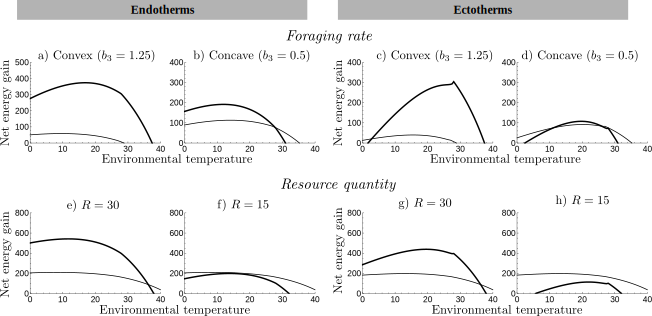
\includegraphics[width=\textwidth]{fig5}
\caption{
    \setstretch{\stretchby}
	Qualitative results on how foraging rate and resource quantity affect the thermal performance curves for small (thin) and large (thick) body sizes.
  We assumed free convection and warm-up starts half an hour after sunrise.
  For a--d, $\tau_f = 1$, ($z = 0.5 \mbox{ or } 2$) .
	For e--h, $b_1 = b_2 = b_3 = 0.75,$ ($z = 0.2 \mbox{ or } 2$)
	Remaining parameters: $\rho = 24, a_2 = 10 a_1$.
	See \cref{table:table1} for units and default parameters.
}
\label{fig5}
\end{figure}


\end{document}
